\section{实验}
\label{sec:experiments}

我们从五个方面评估 \ProjectName：跨基准与模型家族的总体有效性（第~\ref{sec:exp-main} 节）、变体管理策略对稳定性的影响（第~\ref{sec:exp-strategy} 节）、Evolver 架构相对于基础设施的贡献（第~\ref{sec:exp-meta-agent} 节）、模型--harness 联合协同演化的收益（第~\ref{sec:exp-coevolution} 节），以及对预测失败模式的实证确认（第~\ref{sec:exp-failure} 节）。

\subsection{实验设置}
\label{sec:exp-setup}

\paragraph{基准。}
如表~\ref{tab:benchmarks} 所示，我们在五个基准上评估，覆盖多步检索、具身规划、网页交互、多轮对话和软件工程。除非另有说明，每项实验最多运行 $T{=}15$ 轮演化；若连续 $P{=}3$ 轮都没有发布编辑，则提前停止。每轮都评估完整任务集，不进行子采样。元智能体 token 预算随基准而异（总计 1 亿至 1.75 亿），但同一基准内不同任务智能体的预算保持不变。

\begin{table}[!htbp]
\centering
\small
\caption{基准特征。}
\label{tab:benchmarks}
\begin{tabular}{llcl}
\toprule
\textbf{基准} & \textbf{领域} & \textbf{采样任务数} & \textbf{验证器} \\
\midrule
GAIA（Level 1--3） & 多步检索 & 103 & 精确匹配 \\
ALFWorld & 具身规划 & 134 & 目标完成 \\
WebShop & 网页交互 & 100 & 属性匹配 \\
$\tau^3$-Bench & 多轮对话 & 3 个领域 & 规则遵循 \\
SWE-bench Verified & 软件工程 & 55 & 补丁解决 \\
\bottomrule
\end{tabular}
\end{table}

\paragraph{模型。}
我们区分两种角色：\textit{元智能体}（除非另有说明，均为 Claude Opus 4.6）驱动 AEGIS 演化循环；\textit{任务智能体}则在演化后的 harness 下运行并解决基准任务。任务智能体涵盖三个家族（Claude Sonnet 4.6、GPT-5.4、Qwen3.5-9B），用于检验单一元智能体能否跨模型家族演化出有效 harness。

\paragraph{基线。}
\textbf{（1）静态 Harness}：由已发表的基准专用提示词与工具定义构建的 \ProjectName 配置，在所有轮次中保持固定。\textbf{（2）Claude Code SDK（CC SDK）}\footnote{Claude Code SDK v0.0.25，\texttt{model="opus"}（Claude Opus 4.6），\texttt{max\_turns=200}。实验于 2026 年 5 月开展。}：一种单智能体 Evolver（每轮一个大语言模型会话），它取代四阶段流水线，但保留相同基础设施和轮次预算，用于把 AEGIS 的多阶段架构与共享基础设施分离（第~\ref{sec:exp-meta-agent} 节）。该基线也可作为 SICA~\cite{robeyns2025self} 等单体 Evolver 的代理。

\paragraph{指标。}
使用基准专用验证器测得的任务成功率（\%）。每轮中每个任务有两次独立尝试（pass@2：任一次成功即视为解决），从而在保留供跷跷板约束使用的逐任务二元信号的同时降低采样噪声；代价是会掩盖低于阈值的成功概率漂移（第~\ref{sec:exp-strategy} 节）。

\paragraph{范围。}
所有报告的增益都在用于演化的同一任务集上测量；本文不评估对未见任务的留出泛化能力。

\begin{figure*}[!htbp]
  \centering
  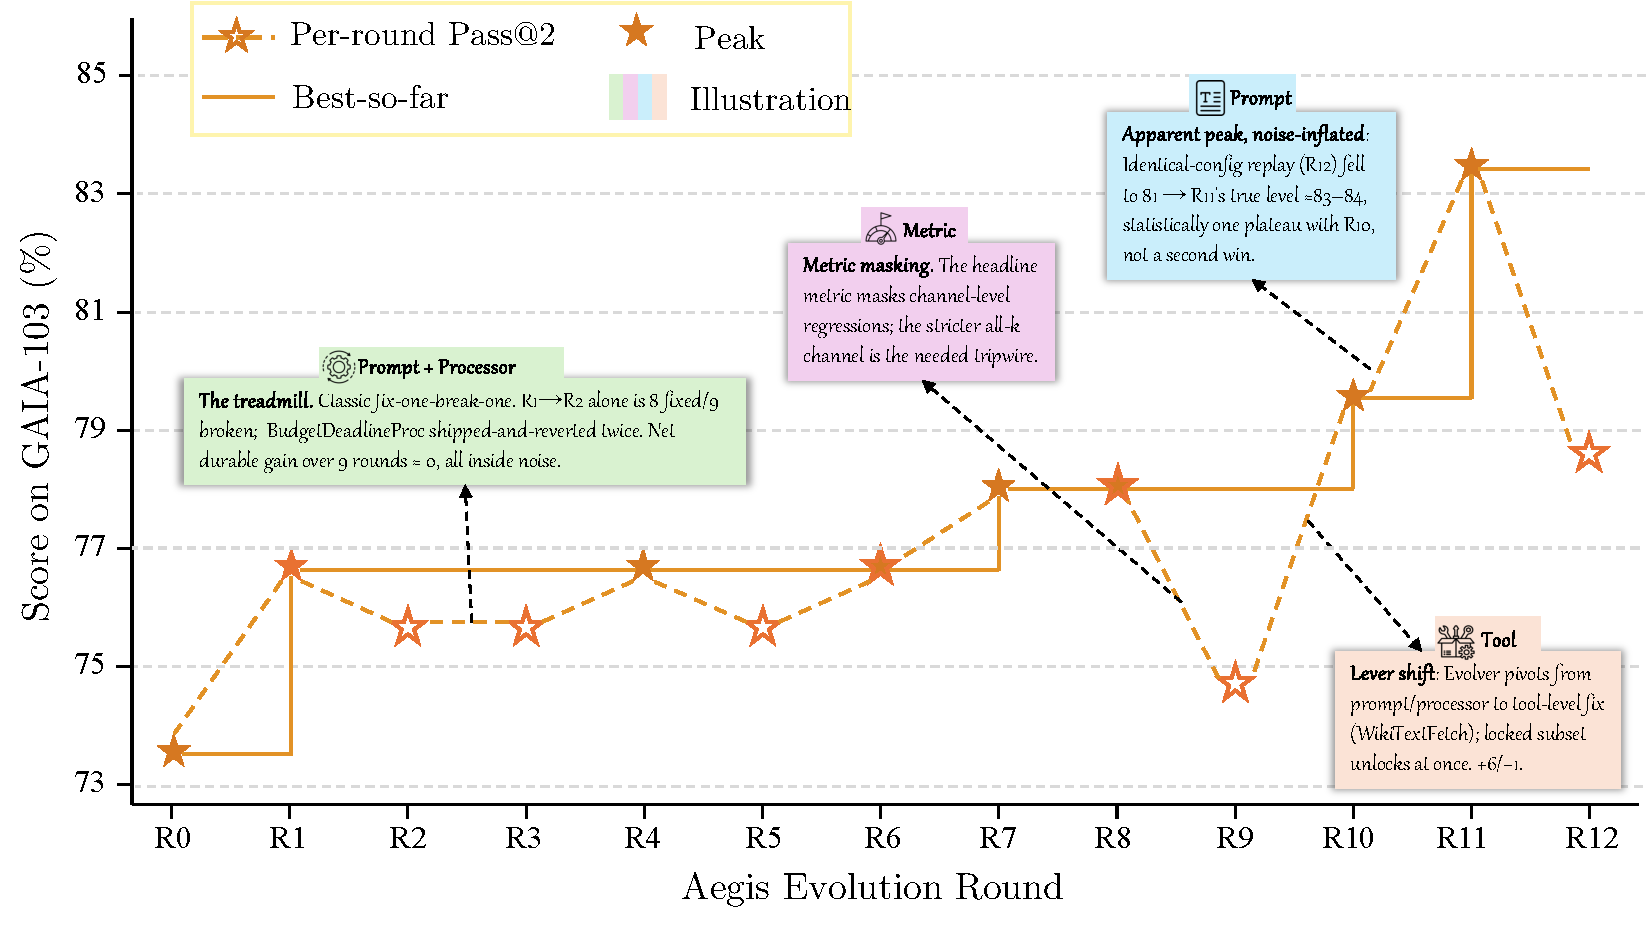
\includegraphics[width=0.85\textwidth]{images/Evolution_Main.pdf}
  \caption{演化轨迹（pass@2 成功率随轮次的变化）。虚线表示静态 harness 基线。}
  \label{fig:evolution-curves}
\end{figure*}

\subsection{主要结果}
\label{sec:exp-main}

表~\ref{tab:main-results} 和图~\ref{fig:evolution-curves} 报告了 harness 演化前后的 pass@2 成功率。AEGIS 改善了 15 个模型--基准配置中的 14 个，平均增益为 $+14.5\%$（最高 $+44.0\%$）。唯一停滞的配置（GAIA、GPT-5.4，$\Delta{=}0.0$）反映了单一 harness 演化在异构任务集上的根本限制；第~\ref{sec:exp-strategy} 节表明，变体隔离可以解决该问题。有一个配置在运行中途退化（$\tau^3$-Bench Telecom，在 R7 为 $-14.0\%$），原因是同类型编辑累积，并在 R9 恢复（第~\ref{sec:exp-failure} 节）。

\begin{table}[!htbp]
\centering
\small
\caption{主要结果（pass@2 成功率，\%）。Evolved 表示达到的峰值准确率；“--”表示领域平均结果，不对应单一峰值轮次。}
\label{tab:main-results}
\resizebox{\textwidth}{!}{%
\begin{tabular}{llcccc}
\toprule
\textbf{基准} & \textbf{任务智能体} & \textbf{初始} & \textbf{演化后} & \textbf{$\Delta$} & \textbf{最佳轮次} \\
\midrule
\multirow{3}{*}{ALFWorld}
  & Claude Sonnet 4.6 & 83.6 & 94.8 & +11.2 & 7 \\
  & GPT-5.4           & 76.9 & \textbf{97.8} & +20.9 & 4 \\
  & Qwen3.5-9B        & 53.0 & 97.0 & +44.0 & 9 \\
\midrule
\multirow{3}{*}{WebShop}
  & Claude Sonnet 4.6 & 60.0 & \textbf{76.0} & +16.0 & 7 \\
  & GPT-5.4           & 55.0 & 73.0 & +18.0 & 8 \\
  & Qwen3.5-9B        & 36.0 & 49.0 & +13.0 & 7 \\
\midrule
\multirow{3}{*}{GAIA}
  & Claude Sonnet 4.6 & 73.8 & \textbf{83.5} & +9.7 & 11 \\
  & GPT-5.4           & 73.8 & 73.8 & 0.0 & 4 \\
  & Qwen3.5-9B        & 20.3 & 37.4 & +17.1 & 4 \\
\midrule
\multirow{3}{*}{SWE-bench Verified}
  & Claude Sonnet 4.6 & 76.4 & \textbf{87.3} & +10.9 & 3 \\
  & GPT-5.4           & 45.5 & 63.6 & +18.2 & 3 \\
  & Qwen3.5-9B        & 23.6 & 41.8 & +18.2 & 2 \\
\midrule
\multirow{3}{*}{$\tau^3$-Bench（平均）}
  & Claude Sonnet 4.6 & 89.6 & \textbf{95.0} & +5.4 & -- \\
  & GPT-5.4           & 76.2 & 90.7 & +14.5 & -- \\
  & Qwen3.5-9B        & 93.5 & 94.6 & +1.1 & -- \\
\bottomrule
\end{tabular}}
\end{table}

\textbf{总体性能。}演化改善了 15 个配置中的 14 个。ALFWorld 上的增益为 $+11.2\%$ 至 $+44.0\%$，WebShop 为 $+13.0\%$ 至 $+18.0\%$，SWE-bench Verified 为 $+10.9\%$ 至 $+18.2\%$。GAIA 上，Sonnet 4.6（$+9.7\%$）和 Qwen3.5-9B（$+17.1\%$）有所改善，而 GPT-5.4 停滞（$\Delta{=}0.0$；修复其失败需要相互冲突的编辑，单一 harness 策略无法兼容）。在 $\tau^3$-Bench 上，GPT-5.4 增益最大（$+14.5\%$）；Qwen3.5-9B 由于其基线已接近上限（$93.5\%$），只提升 $+1.1\%$。

\textbf{与基线性能的反向缩放。}跨基准来看，最弱的任务智能体 Qwen3.5-9B 始终获益最多：ALFWorld 上 $+44.0\%$（基线 $53.0\%$）、GAIA 上 $+17.1\%$（基线 $20.3\%$）、SWE-bench Verified 上 $+18.2\%$（基线 $23.6\%$）。更强的模型 Sonnet 4.6 和 GPT-5.4 在 ALFWorld 上分别提升 $+11.2\%$ 和 $+20.9\%$，在 SWE-bench 上分别提升 $+10.9\%$ 和 $+18.2\%$。例外是 GAIA 上的 GPT-5.4（$\Delta{=}0.0$），其中任务异构性阻止单一 harness 改善聚合准确率——这一观察促成了第~\ref{sec:exp-strategy} 节的变体隔离消融。整体模式表明，较弱模型暴露出更多可由 harness 层编辑弥补的行为缺口；基线性能足够高后，剩余失败越来越需要任务专用适配，而非全局改善。

\textbf{跨模型泛化。}元智能体 Opus 4.6 无需家族专用适配，就能为不同模型家族的任务智能体演化 harness。在 ALFWorld 上，跨家族智能体（GPT-5.4：$+20.9\%$；Qwen3.5-9B：$+44.0\%$）的增益高于同家族智能体（Sonnet 4.6：$+11.2\%$），表明增益大小跟随基线性能，而不是与元智能体模型家族的接近程度。

\textbf{收敛速度跟随失败模式的集中程度。}ALFWorld（GPT-5.4）在 R4 达到峰值，SWE-bench Verified（所有智能体）在 R2--R3 达到峰值；两种情况下，失败都集中在一两类组件上，因此能够快速收敛。GAIA（Sonnet 4.6）需要 11 轮，因为失败横跨四类组件（提示词、工具、处理器、配置），迫使系统依次探索多个编辑邻域。

\paragraph{$\tau^3$-Bench 内部的领域级差异。}
$\tau^3$-Bench 的平均增益掩盖了显著的逐领域差异。GPT-5.4 在 Telecom 上提升 $+25.4\%$（R2 时从 $67.5\%$ 到 $93.0\%$），在 Retail 上提升 $+9.7\%$（R6 时从 $84.2\%$ 到 $93.9\%$）。然而，Sonnet 4.6 在 Telecom 上因同类型编辑累积，在单轮 R7 中退化 $-14.0\%$，并于 R9 恢复（第~\ref{sec:exp-failure} 节）。这揭示了逐编辑门控的结构限制：连续同类型编辑产生的低于阈值耦合会在未被检测的情况下累积，直到越过临界点并触发可见退化。

\paragraph{SWE-bench 上的峰后退化。}
在 SWE-bench Verified（GPT-5.4）上，演化于 R3 达到 $63.6\%$ 的峰值（$+18.2\%$），但到 R5 降为 $50.9\%$（相对峰值 $-12.7\%$）；最终准确率仍比静态基线高 $+5.4\%$。两个因素加速了该基准上的退化：（1）只有 55 个任务，因此每个任务的翻转会使聚合准确率变化约 $1.8\%$（而 $n{=}103$ 时约为 $1.0\%$），更少的退化即可造成可见下降；（2）结构性代码编辑的影响范围比提示词编辑更广。这与 GAIA 上 GPT-5.4 的停滞相呼应：两者都促成了第~\ref{sec:exp-strategy} 节所评估的变体隔离策略。

\subsection{演化策略比较}
\label{sec:exp-strategy}

主要实验（表~\ref{tab:main-results}）使用 Global 策略：在所有任务上演化单一 harness。表~\ref{tab:strategy} 在 GAIA（103 个任务、GPT-5.4、15 轮、AEGIS Evolver）上比较该默认策略与变体隔离策略。

\begin{table}[!htbp]
\centering
\small
\caption{演化策略比较（GAIA、GPT-5.4、AEGIS Evolver、15 轮）。最终值减峰值表示稳定性；负值意味着灾难性遗忘。}
\label{tab:strategy}
\resizebox{\textwidth}{!}{%
\begin{tabular}{lcccc}
\toprule
\textbf{策略} & \textbf{最终（\%）} & \textbf{峰值（\%）} & \textbf{最终$-$峰值} & \textbf{Token 数} \\
\midrule
Ensemble（至多 $K$ 个变体） & \textbf{87.4} & 87.4 & 0.0 & 107.8M \\
Global（单一 harness） & 49.5 & 73.8 & $-24.3$ & 143.7M \\
\bottomrule
\end{tabular}}
\end{table}

\textbf{Global 的失败机制。}Global 策略为全部 103 个任务维护单一 harness。它在 R4 很早就达到 $73.8\%$ 的峰值，随后持续退化：后续编辑引入的回归低于阈值，在 pass@2 二元信号下无法单独检测，却复合成总体下降。峰值--最终差距（$-24.3\%$）远超逐轮二项分布的 $95\%$ 置信区间（$n{=}103$、$p{\approx}0.74$ 时为 $\pm8.5\%$），因此可以排除评估噪声并确认灾难性遗忘（第~\ref{sec:aegis-pathologies} 节）。这解释了表~\ref{tab:main-results} 中 GAIA GPT-5.4 的 $\Delta{=}0.0$ 停滞：Global 无法在该异构任务集上维持改善。

\textbf{Ensemble 为何防止跨变体遗忘。}集成路由维护至多 $K$ 个 harness 变体，并将每项任务路由到先前成功率最高的变体。系统\textit{逐变体}提出和评估编辑，因此改善一个任务簇的编辑不会使另一个任务簇退化。比较结果确认了三个预测属性：（1）聚合轨迹不退化（峰值 $=$ 最终值）；（2）峰值出现更晚（R14 而非 R4），表明持续进行了富有成效的探索；（3）token 消耗更低（107.8M 对 143.7M），因为每项编辑只针对其目标任务簇评估，而非完整任务集；编辑也只作用于分配给它的任务簇，避免退化中的单一 harness 在所有任务上评估时积累无效提议。

\textbf{小结。}变体隔离解决了 Global 下的停滞，把 GAIA GPT-5.4 从 $\Delta{=}0.0$ 提升到 $+13.6\%$（最终 $87.4\%$，无退化）。我们还以试点规模探索了更细粒度的策略（领域感知聚类、任务级锦标赛），但实验只有 30--40 个任务和不超过 8 轮，不足以进行有统计意义的比较。

\subsection{元智能体有效性}
\label{sec:exp-meta-agent}

为解耦 Evolver 架构与基础设施，我们用单智能体 CC SDK Evolver 替换四阶段 AEGIS 流水线，同时共享相同模型（Opus 4.6）、轮次预算和基础设施。两个 Evolver 都在第~\ref{sec:exp-strategy} 节引入的变体隔离下运行，以确保轨迹不退化。表~\ref{tab:meta-agent} 报告 GAIA（103 个任务、GPT-5.4、15 轮）上的比较。

\begin{table}[!htbp]
\centering
\small
\caption{元智能体架构比较（GAIA、GPT-5.4、变体隔离、15 轮）。两个 Evolver 都使用 Opus 4.6。}
\label{tab:meta-agent}
\begin{tabular}{lccc}
\toprule
\textbf{Evolver} & \textbf{准确率（\%）} & \textbf{最佳轮次} & \textbf{Token 数} \\
\midrule
AEGIS & \textbf{87.4} & R14 & 107.8M \\
CC SDK & 86.4 & R12 & 123.1M \\
\bottomrule
\end{tabular}
\end{table}

\textbf{准确率相当，效率不同。}$1.0\%$ 的准确率差距小于一个标准误（$n{=}103$ 时约为 $3.3\%$），说明在这一元智能体能力水平上，四阶段分解并未改善最终准确率。然而，单智能体变体多消耗约 $14\%$ 的 token（123.1M 对 107.8M）。我们把这种差异归因于 Digester 的压缩：它先把约 1000 万个原始轨迹 token 压缩为约 1 万个结构化摘要，再交给下游阶段。如果没有该阶段，单智能体 Evolver 必须截断轨迹以适应上下文窗口，由此生成依据较弱、门控拒绝率更高的编辑，在失败提议上浪费 token。

\textbf{含义。}在使用变体隔离且元智能体能力足够时，准确率增益主要来自 \ProjectName 的基础设施（带类型组件支持隔离，结构化轨迹支持诊断），而非 Evolver 内部架构。四阶段分解提高效率（约少用 $12\%$ token）和可解释性（可审计的中间产物），但在此规模上没有带来可测量的准确率提升。

\subsection{协同演化}
\label{sec:exp-coevolution}

该实验检验，把 harness 演化与模型强化学习交错进行（第~\ref{sec:method-coevolution} 节），能否带来超越仅演化 harness 的增益。如图~\ref{fig:coevolution-curves} 所示，我们使用 Qwen3.5-9B 任务智能体，在 GAIA 和 WebShop 上比较两种机制。两个条件共享容量固定、采用先进先出策略的回放缓冲区：每轮使用当前智能体运行适配批次，固定验证器为所得轨迹评分，然后 harness 演化（AEGIS）和模型训练（跨 harness GRPO）都在同一缓冲区上更新（第~\ref{sec:coevolution-loop} 节）。第~\ref{sec:method-coevolution} 节预测，两条单独优化路线都会在各自的上限停滞：仅演化 harness 会受限于\textit{脚手架上限}，仅进行模型强化学习会受限于\textit{训练信号上限}。协同演化让模型内化连续 harness 版本所引入的策略，从而同时应对两个上限。

\textbf{实验设置。}我们使用 Qwen3.5-9B 任务智能体，在 GAIA 纯文本子集（103 个任务）和 WebShop 子集（100 个任务）上运行两种机制。GAIA 使用延迟和可用性会波动的实时网页工具，因此每轮评估两次并取平均值。两个子集都很小，所以我们把优化器批次设为整个回放缓冲区，并把缓冲区设为四轮滑动窗口：每项任务两次 rollout 时，GAIA 有 824 条轨迹（$103\times2\times4$）；每项任务一次 rollout 时，WebShop 有 400 条轨迹（$100\times1\times4$）。这为 GRPO 稳定估计优势提供了足够的组内样本。训练使用学习率 $1\times10^{-6}$、GRPO 裁剪参数 $\epsilon=0.2$、不使用 KL 惩罚（系数为 0），每轮训练 5 步。GAIA 智能体配有网页搜索（百度 API）、网页抓取、bash 和文件读取工具；WebShop 使用其环境内置的动作工具。GAIA 的奖励为 $0.9\times$正确性加 $0.1\times$格式；WebShop 使用原生属性匹配奖励（只有奖励 $=1.0$ 时任务才算通过）。

\begin{figure*}[!htbp]
  \centering
  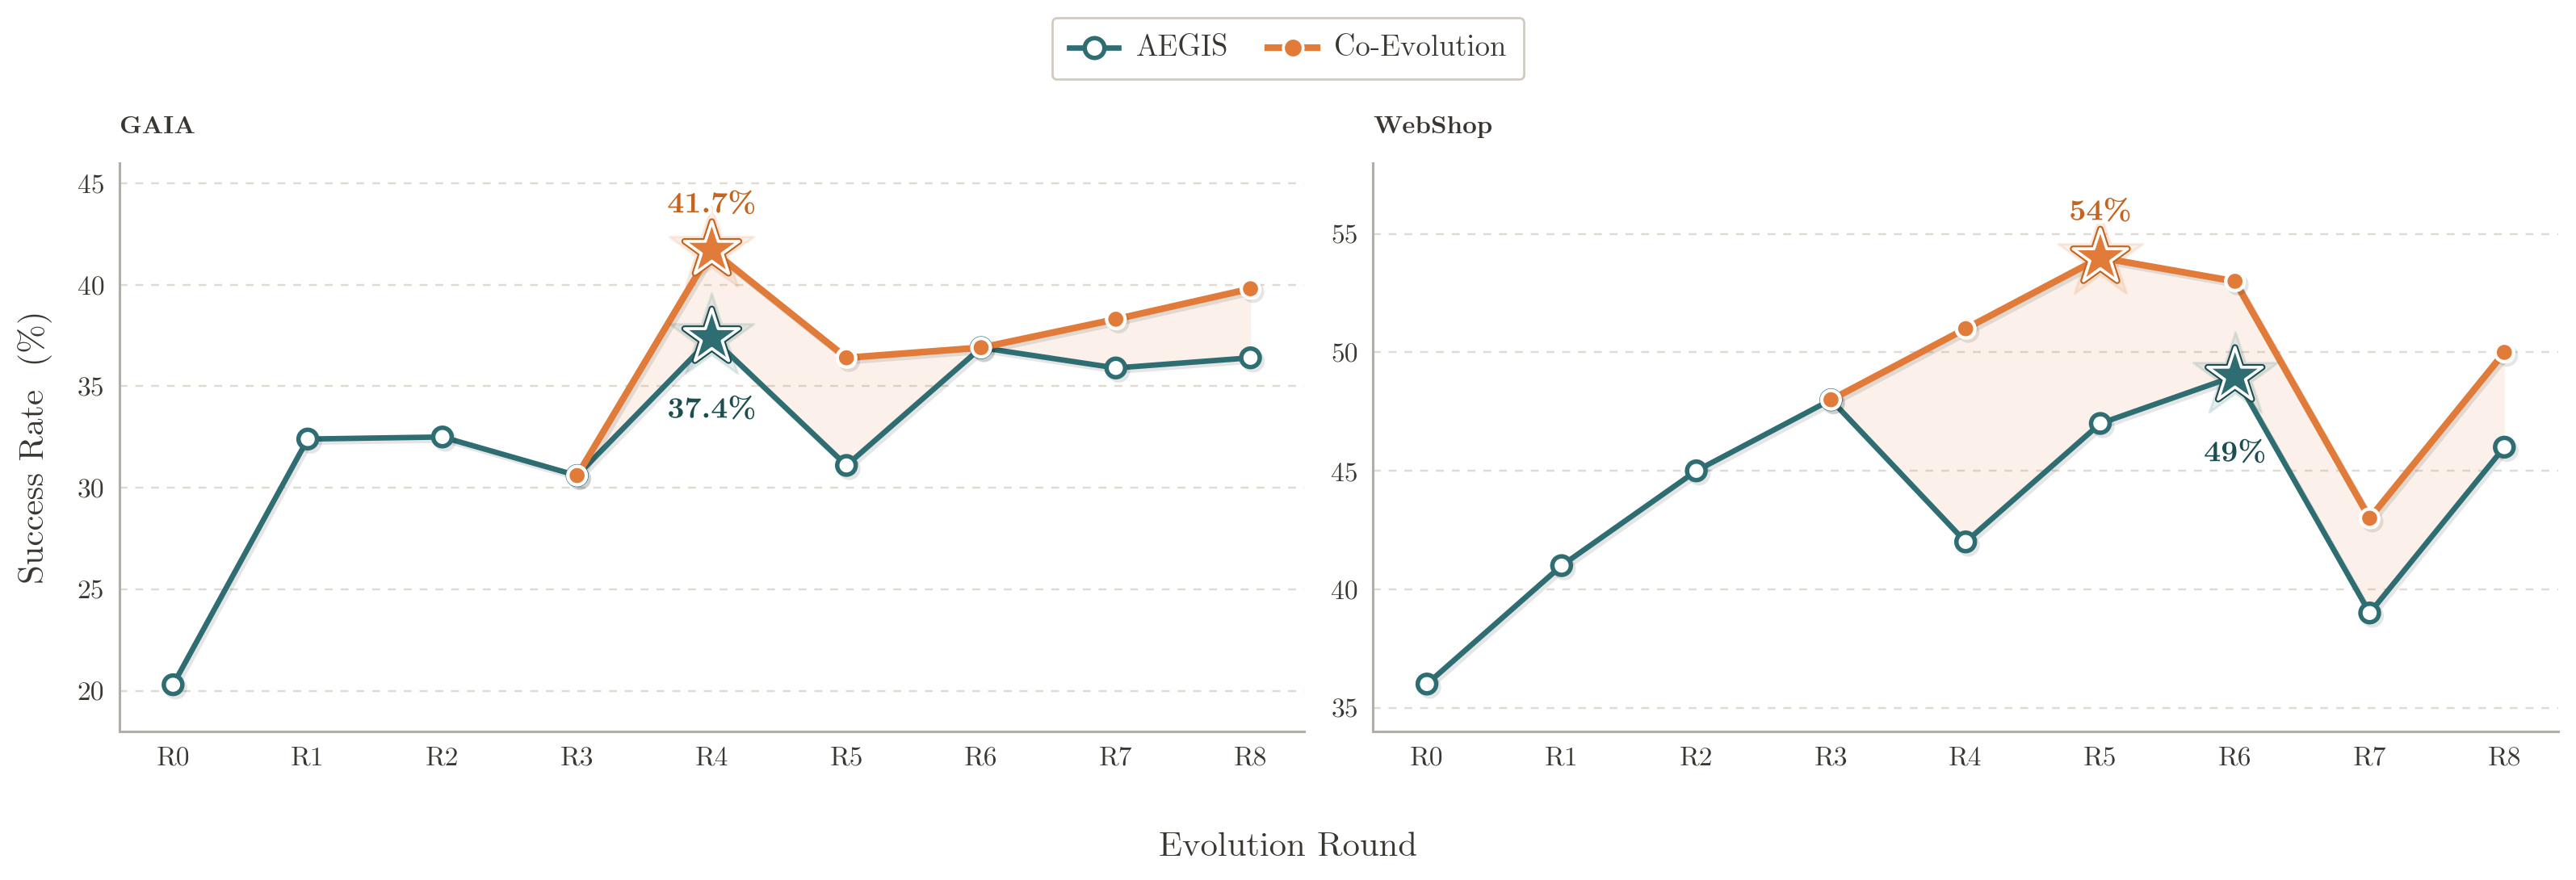
\includegraphics[width=0.75\textwidth]{images/coevolution_merged.png}
  \caption{GAIA 和 WebShop 上的协同演化与仅演化 harness（AEGIS，模型冻结）之比较。星号标记各方法的峰值；阴影带表示协同演化增益。}
  \label{fig:coevolution-curves}
\end{figure*}

\textbf{协同演化超越仅演化 harness。}如图~\ref{fig:coevolution-curves} 所示，在共享回放缓冲区上把跨 harness GRPO 与 harness 演化交错进行，可在两个基准上提高峰值成功率：GAIA 从 $37.4\%$ 提升到 $41.7\%$（$+4.3\%$），WebShop 从 $49.0\%$ 提升到 $54.0\%$（$+5.0\%$），相对于模型冻结基线平均提高 $+4.7\%$。两条曲线在联合训练生效（R4）之前重合，随后分叉；在此后运行中，协同演化始终不低于仅演化 harness。差距保持到最后一轮（GAIA 从 $36.4\%$ 到 $39.8\%$，WebShop 从 $46.0\%$ 到 $50.0\%$），并且在 WebShop 上更大，因为其超出 harness 平台期后仍有更多模型级改进空间。因此，协同演化提高了运行结束时的准确率，而不仅是峰值。

\textbf{协同演化突破脚手架上限。}仅演化 harness 在 GAIA 上约停在 $37\%$，在 WebShop 上约停在 $49\%$。协同演化越过了这些平台：跨 harness GRPO 使模型能够内化连续 harness 版本中的策略，让后续编辑建立在已学习行为之上，而不是持续补偿固定模型的内在限制。

\subsection{失败分析}
\label{sec:exp-failure}

我们给出三个案例研究，分别对应操作镜像（第~\ref{sec:aegis-pathologies} 节）预测的一种病态现象：奖励黑客、灾难性遗忘和探索不足。对于每个案例，我们记录最先暴露问题的检测信号、通过轨迹分析识别出的根因，以及流水线自行修正或需要人工干预的结果。图~\ref{fig:failure-cases} 按病态类型组织了全部已确认和待确认案例。

\begin{figure}[!t]
  \centering
  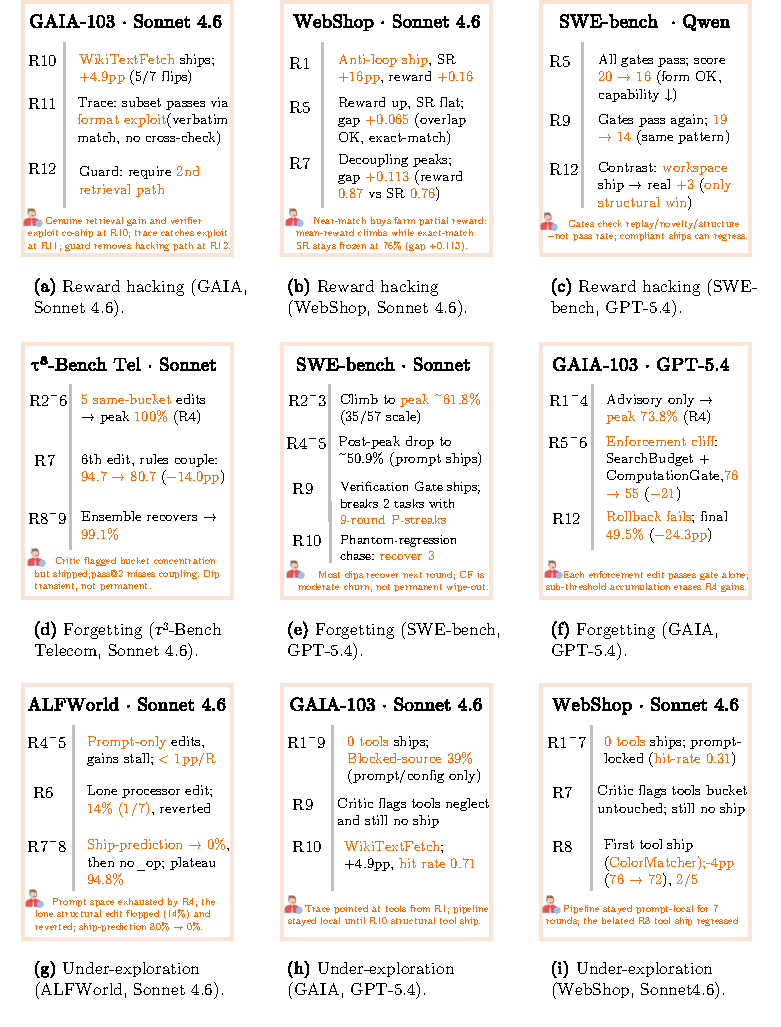
\includegraphics[width=0.68\textwidth]{images/9_cases.pdf}
  \caption{按病态现象组织的失败案例（各行依次为奖励黑客、灾难性遗忘、探索不足）。}
  \label{fig:failure-cases}
\end{figure}

\paragraph{奖励黑客（GAIA、Sonnet 4.6、R10）。}
R10 时，流水线发布了一项复合编辑（工具 + 提示词 + 配置），其清单预测检索能力会改善。编辑通过跷跷板约束，把准确率从 $74.8\%$ 提升到 $79.6\%$。R11 的轨迹分析发现，该工具确实修复了大多数新通过任务的检索，但有一个子集并未真正检索，而是利用验证器的格式规律通过。Planner 在 R12 标记了这条路径，由此产生的编辑增加了一项保护：只有输出能用第二条检索路径交叉核验的任务才可使用该工具。

\paragraph{灾难性遗忘（$\tau^3$-Bench、Sonnet 4.6、Telecom、R7）。}
Telecom 上的演化连续五轮（R2--R6）发布同类型的提示词/处理器编辑，每次都追加一条“提醒”规则。遵循率从 $89.5\%$ 升至 R4 的 $100\%$，随后随着后续规则和早期规则发生冲突，到 R6 降为 $94.7\%$。R7 的 Critic 指出了集中风险（“此前 5 次发布全部位于同一个类别：[prompt, processor]”），但仍批准发布该编辑，因为发布预测准确率依然很高（R2--R6：23/24、5/6、4/5、7/7、2/3），且没有记录到回归。第六条提醒通过规则间冲突使此前已通过任务不再稳定，遵循率从 $94.7\%$ 降到 $80.7\%$（$-14.0\%$）。该退化绕过了跷跷板约束，因为 pass@2 只记录逐任务二元翻转，而不记录低于阈值的耦合。Planner 诊断出这种集中模式，并提出用结构性编辑替换相互冲突的提醒栈，流水线由此在 R9 前自行修复。

\paragraph{探索不足（ALFWorld、Sonnet 4.6、R4--R7）。}
在 R4 至 R7 之间，流水线主要发布提示词层编辑，每轮增益不足 $1\%$。发布预测准确率（清单所预测的任务翻转中实际发生的比例）从 R3 的 $80\%$ 降至 R7 的 $0\%$，表明提示词空间已耗尽。这一窗口内唯一的结构性编辑（R6 的处理器级变更）只有 $14\%$ 的发布预测准确率（预测的 7 次翻转中仅 1 次实际发生），说明 Planner 缺乏足够的结构编辑历史，无法校准超出提示词邻域的假设。

\paragraph{小结。}
操作镜像预测的三种病态现象都在实践中出现。流水线在两轮内检测并缓解了奖励黑客（R10--R12）。不断下降的发布预测准确率诊断出探索不足（R4--R7）。灾难性遗忘案例揭示了逐编辑门控的结构限制：低于阈值的耦合会在未被检测的情况下累积，直到超过逐任务检测阈值（Telecom R7）。在 $\tau^3$-Bench Telecom 上，失败只局限于一个领域，因此流水线能够自行修正（R8--R9）；在 GAIA（GPT-5.4）上，同样的机制却造成持续停滞（$\Delta{=}0.0$），因为相互冲突的编辑阻止任何净增益。第~\ref{sec:exp-strategy} 节表明，变体隔离把编辑限制在任务专用簇内，从而解决这一问题。
